The aim of this project was to develop a computer graphics application combining several state-of-the-art techniques into a beautiful world.
\begin{figure}[H]
  \centering
  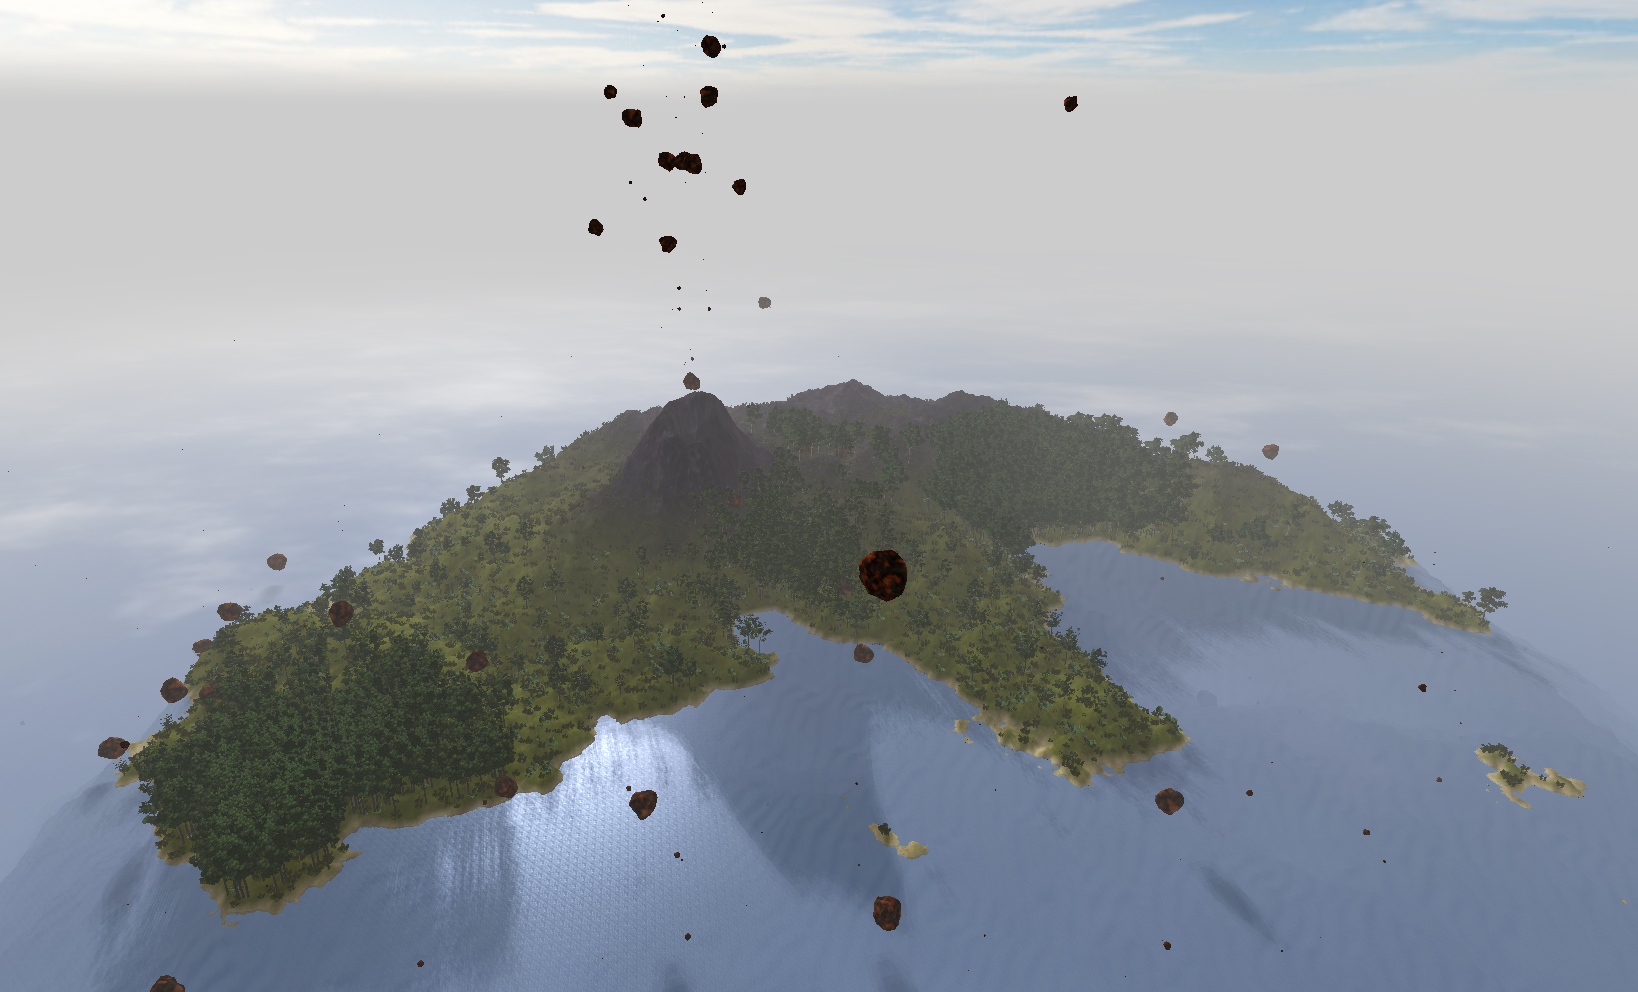
\includegraphics[width=1.0\linewidth]{images/frontImage.jpg}
  \caption[A beautiful world.]{A beautiful world. Containing 3000 trees and 13000 bushes, and a terrain with a vertex density of 5.5.}
  \label{fig:beautifulIsland}
\end{figure}%

During the project a general framework for building games/simulations was developed, using C++11 template programming to provide an easily used Entity System-architecture to manage in-game objects. A rendering system capable of handling large amount of objects without any direct optimizations was also developed alongside the Entity System. The rendering system can manage rendering of large numbers of objects, as well as high quality real-time shadows cast by objects and terrain. A rudimentary world generator based on simplex noise for the terrain generation, and rejection sampling based growth placement.


The project was performed as a part of the course TSBK03 - Techniques for advanced computer games. The code is written in C++11 and GLSL version 150. We use Qt 5.1 as OpenGL wrapper and context provider and OpenCV for some mathematical operations and filtering.